
\documentclass[journal=inoraj,manuscript=article]{achemso}
\usepackage[version=3]{mhchem} % Formula subscripts using \ce{}
\usepackage[T1]{fontenc}       % Use modern font encodings
\usepackage{color}
\usepackage{subcaption}
\usepackage{epstopdf}
\usepackage{epsfig}
\usepackage{graphicx}
%\usepackage[format=hang,singlelinecheck=0,font={sf,small},labelfont=it]{subfig}
\usepackage{caption}
\usepackage{bm}
\usepackage{mciteplus}
\setkeys{acs}{articletitle = true}

\title{EDA analysis SHE}
\author{Leonardo Belpassi}

\author{Loriano Storchi}
\date{November 2022}

\begin{document}

\maketitle

\section{Introduction}

\section{Theoretical background and computational details}

Here some details and a test using ADF vs light atom

\section{A case study the AuX+ (X=Hg, Pb, Rn, Cn, Fl, Og) systems  }

Insert basis set and fitting set used 

\begin{table}[!h]
\begin{tabular}{lrrrrrr}
\hline
                       & AuHg$^+$ & AuCn$^+$ & AuPb$^+$  & AuFl$^+$ & AuRn$^+$ & AuOg$^+$ \\ \hline
\hline
$\Delta E_{int}$       & -51.1341 & -35.1953 & -106.0481 & -65.6807 & -47.4012 & -69.6545 \\ \hline
$\Delta E_{ETS-Pauli}$ &  80.4823 &  79.0281 &  115.7724 &  72.1223 &  85.5963 &  81.6895 \\ \hline
$\Delta E_{exc}$       & -25.9427 & -24.3970 &  -31.8787 & -19.9776 & -24.0878 & -23.3315 \\ \hline
$\Delta E_{Pauli}$     &  54.5396 &  54.6311 &   83.8937 &  52.1447 &  61.5084 &  58.3580 \\ \hline
$\Delta E_{Elect}$     & -42.5393 & -39.3235 &  -65.0604 & -39.1422 & -45.6129 & -46.2992 \\ \hline
$\Delta E_{orb}$       & -63.1344 & -50.5030 & -124.8815 & -78.6832 & -63.2968 & -81.7133 \\ \hline
$\Delta E_1$           & -54.2088 & -38.3577 & -110.5783 & -68.6034 & -49.8713 & -71.7696 \\ \hline
$\Delta E_2$           &  -4.3425 &  -5.5161 &   -2.5708 &  -4.5726 &  -6.0586 &  -4.0202 \\ \hline
$\Delta E_3$           &  -1.0651 &  -2.4930 &   -6.2776 &  -1.4079 &  -4.0528 &  -3.5042 \\ \hline
$\Delta E_4$           &  -1.3728 &  -0.8403 &   -3.1012 &  -1.7332 &  -2.5051 &  -1.4569 \\ \hline
$\Delta E_5$           &  -0.8896 &  -1.6396 &   -0.9819 &  -0.4289 &  -0.1444 &  -0.3208 \\ \hline
$\Delta E_6$           &  -0.4682 &  -0.0176 &   -0.1823 &  -0.0551 &  -0.1193 &  -0.1734 \\ \hline
\end{tabular}
\caption{EDA analysis for AuX$^+$ systems}
\end{table}

\begin{table}[!h]
\begin{tabular}{lrrrrrr}
\hline
                 & AuHg$^+$  & AuCn$^+$  & AuPb$^+$  & AuFl$^+$  & AuRn$^+$  & AuOg$^+$ \\ \hline
\hline
$CT_{nocv1}$     &  0.477012 &  0.361730 &  0.963528 &  0.714536 &  0.490026 &  0.686910 \\ \hline
$CT_{nocv2}$     &  0.000208 & -0.052032 & -0.093912 & -0.027708 & -0.023532 & -0.024638 \\ \hline
$CT_{nocv3}$     & -0.006694 &  0.002634 & -0.055482 & -0.031918 &  0.003218 &  0.006910 \\ \hline
$CT_{nocv4}$     & -0.001326 & -0.006906 & -0.015444 & -0.008188 & -0.007912 & -0.014378 \\ \hline
$CT_{nocv5}$     &  0.002366 &  0.000786 &  0.006334 &  0.003400 & -0.012522 & -0.018664 \\ \hline
$CT_{nocv6}$     & -0.001138 & -0.004616 & -0.003668 & -0.002654 & -0.003216 & -0.002708 \\ \hline
$CT_{tot}$       &  0.435710 &  0.303804 &  0.799147 &  0.651476 &  0.450352 &  0.632027 \\ \hline
$CT_{tot ortho}$ &  0.461715 &  0.303098 &  0.800922 &  0.648890 &  0.442308 &  0.633309 \\ \hline
\end{tabular}
\caption{NOCV CT analysis for AuX$^+$ system}
\end{table}



\begin{figure}[!h]
\includegraphics[angle=-90,width=0.80\textwidth]{./AuHg+/cd.pdf}
\caption{CD curve for AuHg+ system}
\end{figure}

\begin{figure}[!h]
    \centering
    \centering
    \begin{subfigure}[t]{0.30\textwidth}
        \centering
        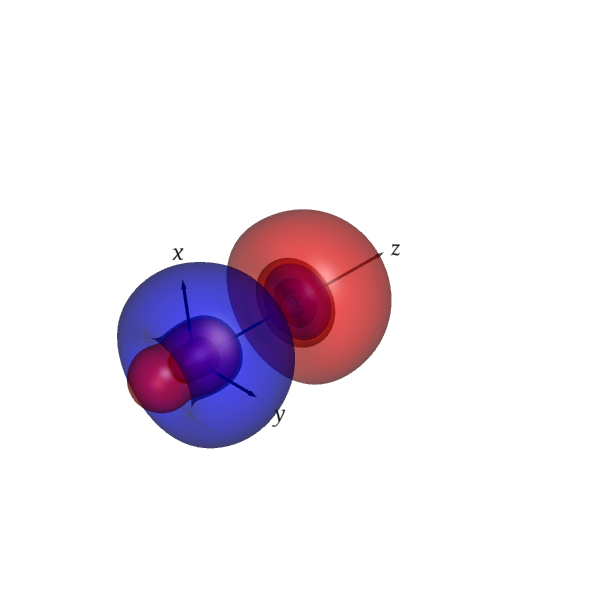
\includegraphics[width=0.80*\linewidth]{./AuHg+/diff_tot.png} 
        \caption*{\ \ \ \ \ \ \ \ $\Delta \rho'$} 
    \end{subfigure}
    \hfill
 
    \vspace{0.0cm}
    \begin{subfigure}[t]{0.30\textwidth}
        \centering
        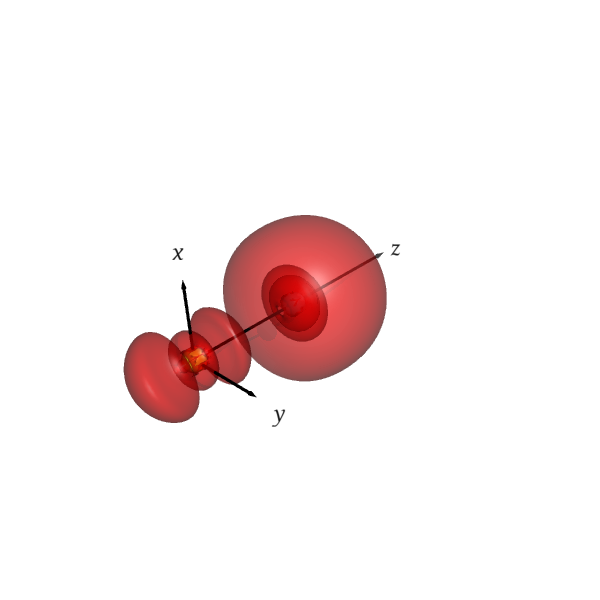
\includegraphics[width=\linewidth]{./AuHg+/nocv-1.png} 
        \caption*{\ \ \ \ \ \ \ \ $|\varphi_{-1}|^2$} 
    \end{subfigure}
    \hfill
    \begin{subfigure}[t]{0.30\textwidth}
        \centering
        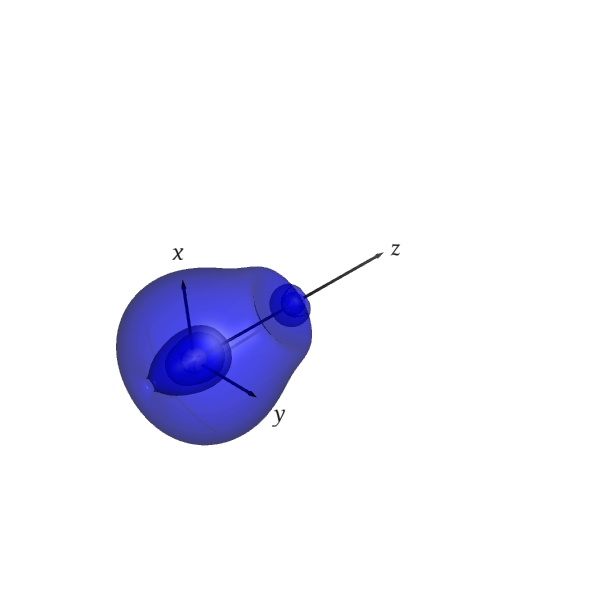
\includegraphics[width=\linewidth]{./AuHg+/nocv+1.png} 
        \caption*{\ \ \ \ \ \ \ \ $|\varphi_{+1}|^2$} 
    \end{subfigure}
    \hfill
    \begin{subfigure}[t]{0.30\textwidth}
        \centering
        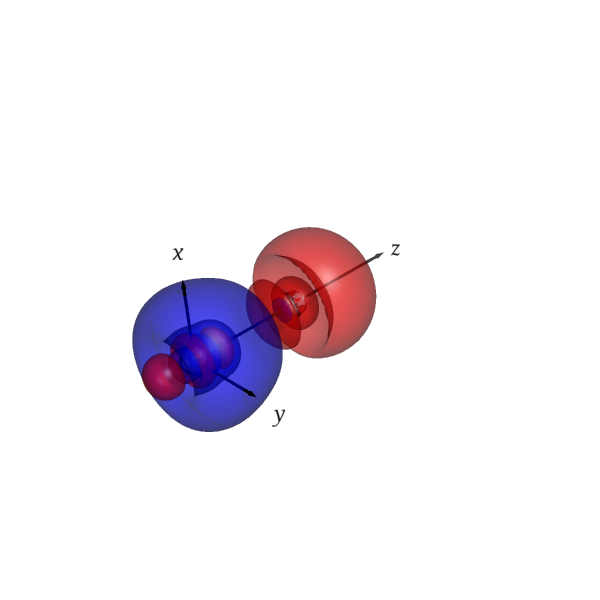
\includegraphics[width=\linewidth]{./AuHg+/pair1.png} 
        \caption*{\ \ \ \ \ \ \ \ $\Delta \rho'_1$} 
    \end{subfigure}

    \vspace{0.0cm}
    \begin{subfigure}[t]{0.30\textwidth}
        \centering
        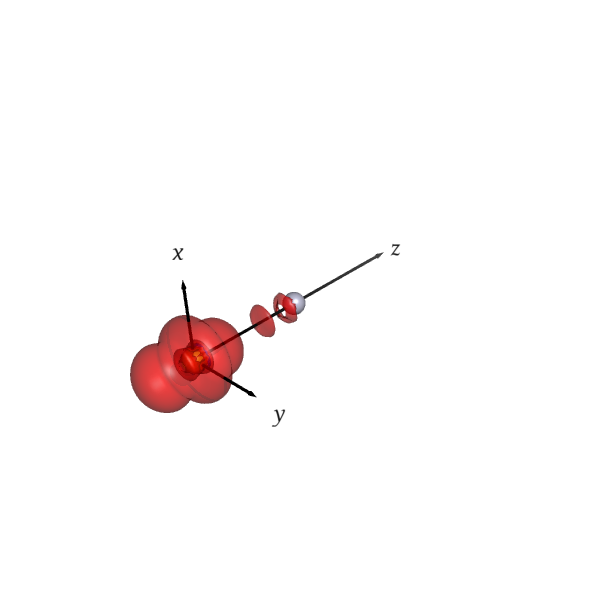
\includegraphics[width=\linewidth]{./AuHg+/nocv-3.png}
        \caption*{\ \ \ \ \ \ \ \ $|\varphi_{-2}|^2$}
    \end{subfigure}
    \hfill
    \begin{subfigure}[t]{0.30\textwidth}
        \centering
        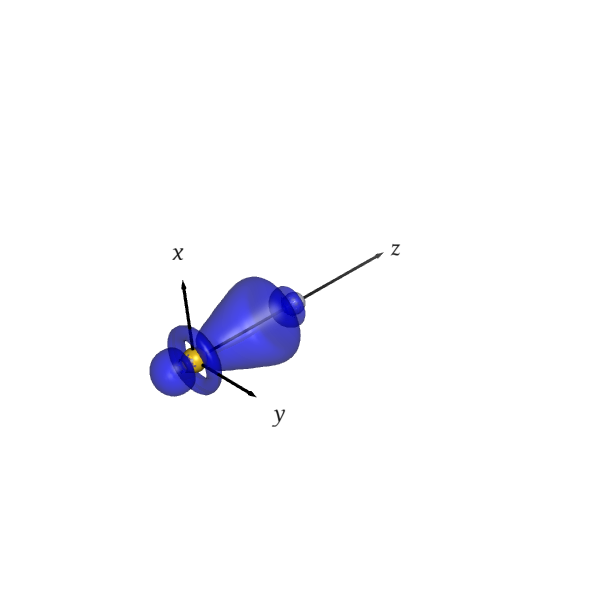
\includegraphics[width=\linewidth]{./AuHg+/nocv+3.png}
        \caption*{\ \ \ \ \ \ \ \ $|\varphi_{+2}|^2$}
    \end{subfigure}
    \hfill
    \begin{subfigure}[t]{0.30\textwidth}
        \centering
        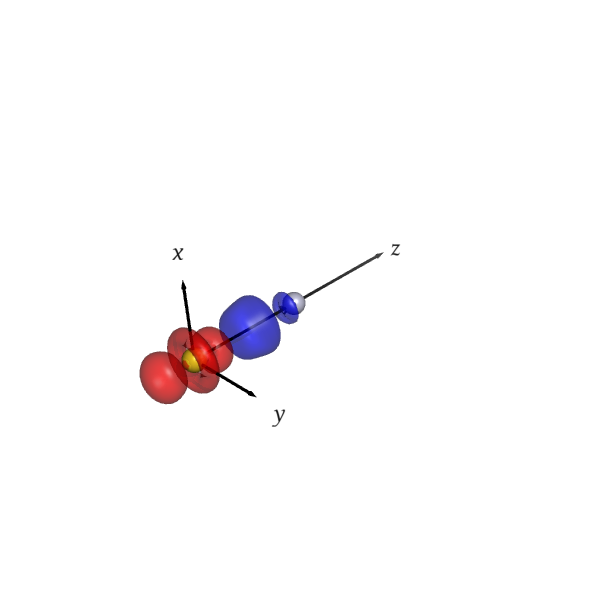
\includegraphics[width=\linewidth]{./AuHg+/pair3.png} 
        \caption*{\ \ \ \ \ \ \ \ $\Delta \rho'_2$} 
    \end{subfigure}

    \vspace{0.0cm}
    \begin{subfigure}[t]{0.30\textwidth}
        \centering
        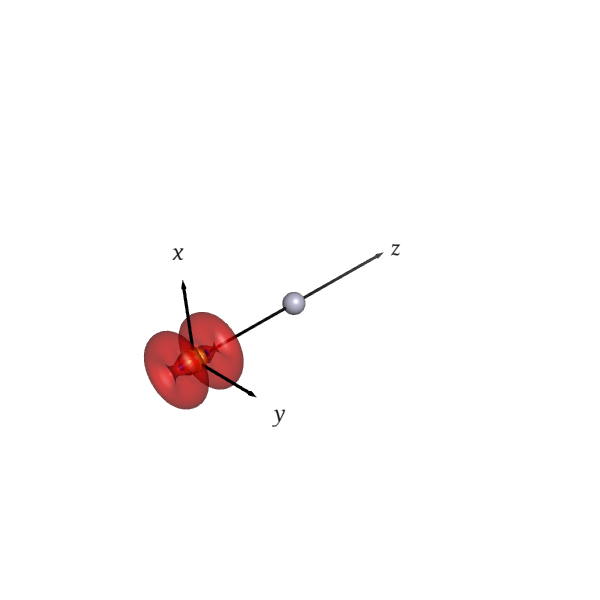
\includegraphics[width=\linewidth]{./AuHg+/nocv-5.png} 
        \caption*{\ \ \ \ \ \ \ \ $|\varphi_{-3}|^2$} 
    \end{subfigure}
    \hfill
    \begin{subfigure}[t]{0.30\textwidth}
        \centering
        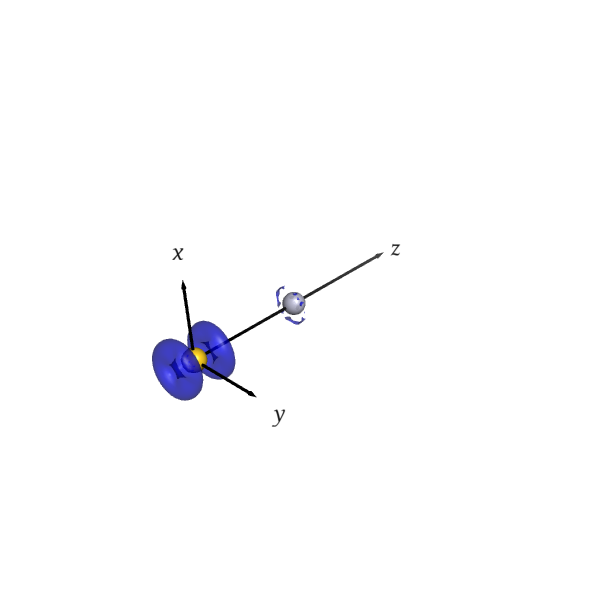
\includegraphics[width=\linewidth]{./AuHg+/nocv+5.png} 
        \caption*{\ \ \ \ \ \ \ \ $|\varphi_{+3}|^2$} 
    \end{subfigure}
    \hfill
    \begin{subfigure}[t]{0.30\textwidth}
        \centering
        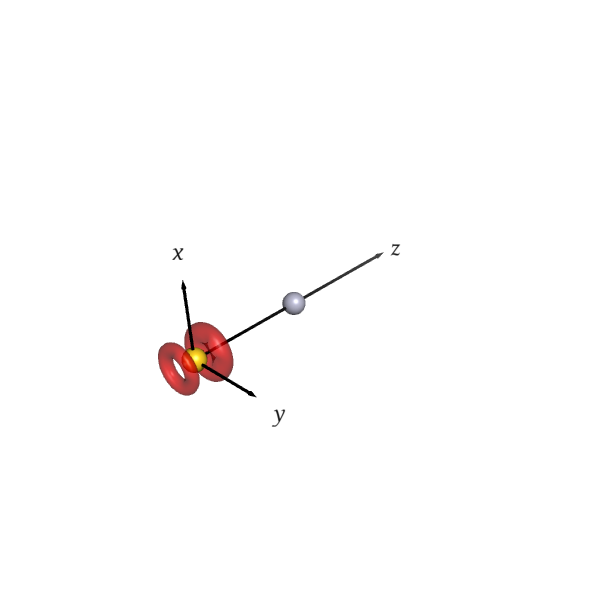
\includegraphics[width=\linewidth]{./AuHg+/pair5.png} 
        \caption*{\ \ \ \ \ \ \ \ $\Delta \rho'_3$} 
    \end{subfigure}

\caption{NOCV pairs for AuHg+ system}
\end{figure}


\begin{figure}[!h]
\includegraphics[angle=-90,width=0.80\textwidth]{./AuCn+/cd.pdf}
\caption{CD curve for AuCn+ system}
\end{figure}
\begin{figure}[!h]
    \centering
    \centering
    \begin{subfigure}[t]{0.33\textwidth}
        \centering
        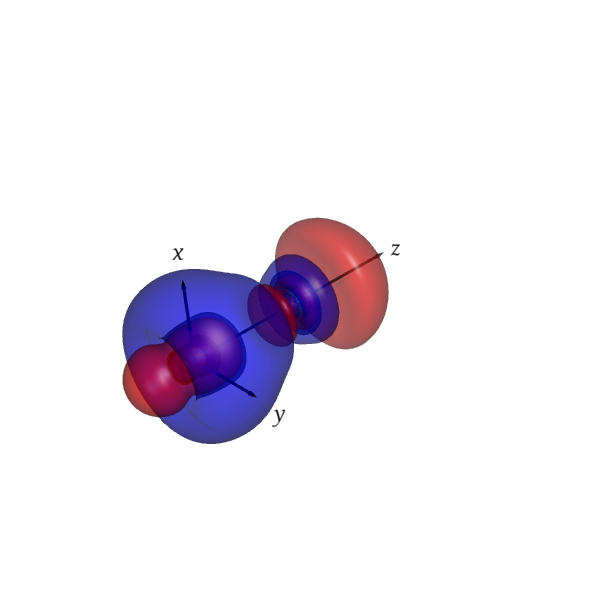
\includegraphics[width=\linewidth]{./AuCn+/diff_tot.png} 
        \caption*{\ \ \ \ \ \ \ \ $\Delta \rho'$} 
    \end{subfigure}
    \hfill
 
    \vspace{0.0cm}
    \begin{subfigure}[t]{0.32\textwidth}
        \centering
        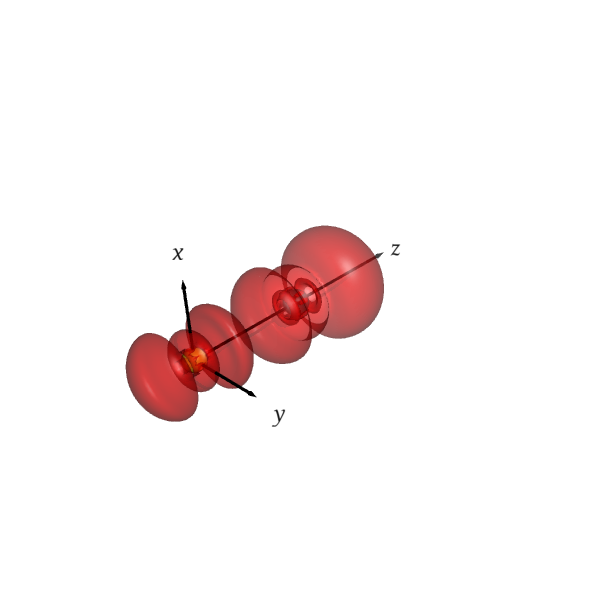
\includegraphics[width=\linewidth]{./AuCn+/nocv-1.png} 
        \caption*{\ \ \ \ \ \ \ \ $|\varphi_{-1}|^2$} 
    \end{subfigure}
    \hfill
    \begin{subfigure}[t]{0.32\textwidth}
        \centering
        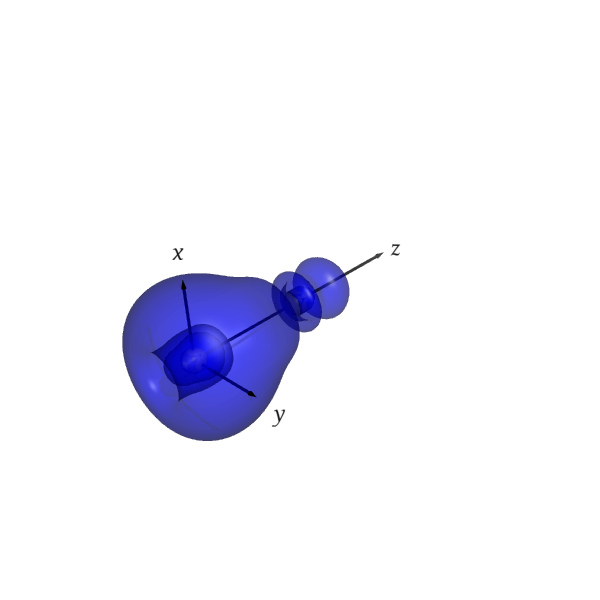
\includegraphics[width=\linewidth]{./AuCn+/nocv+1.png} 
        \caption*{\ \ \ \ \ \ \ \ $|\varphi_{+1}|^2$} 
    \end{subfigure}
    \hfill
    \begin{subfigure}[t]{0.32\textwidth}
        \centering
        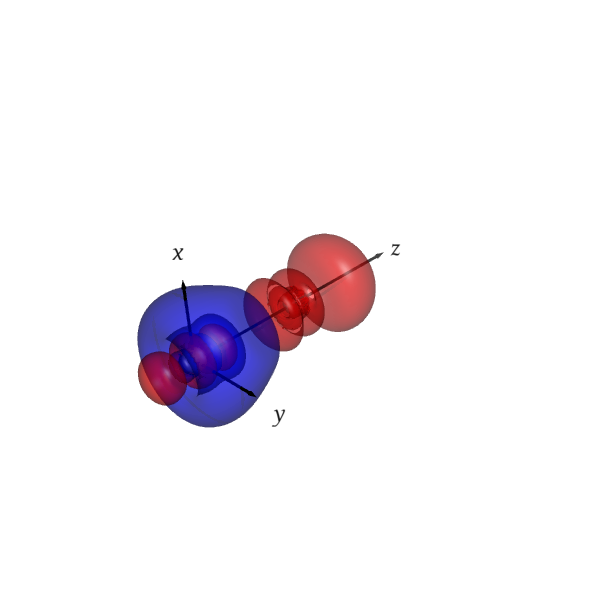
\includegraphics[width=\linewidth]{./AuCn+/pair1.png} 
        \caption*{\ \ \ \ \ \ \ \ $\Delta \rho'_1$} 
    \end{subfigure}

    \vspace{0.0cm}
    \begin{subfigure}[t]{0.32\textwidth}
        \centering
        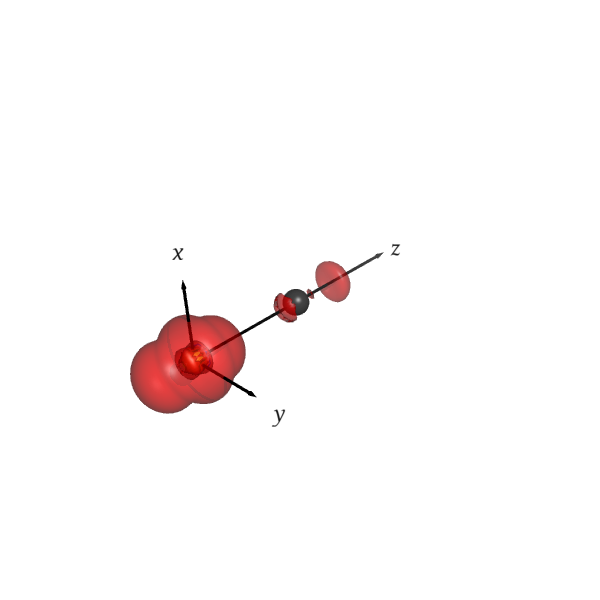
\includegraphics[width=\linewidth]{./AuCn+/nocv-3.png}
        \caption*{\ \ \ \ \ \ \ \ $|\varphi_{-2}|^2$}
    \end{subfigure}
    \hfill
    \begin{subfigure}[t]{0.32\textwidth}
        \centering
        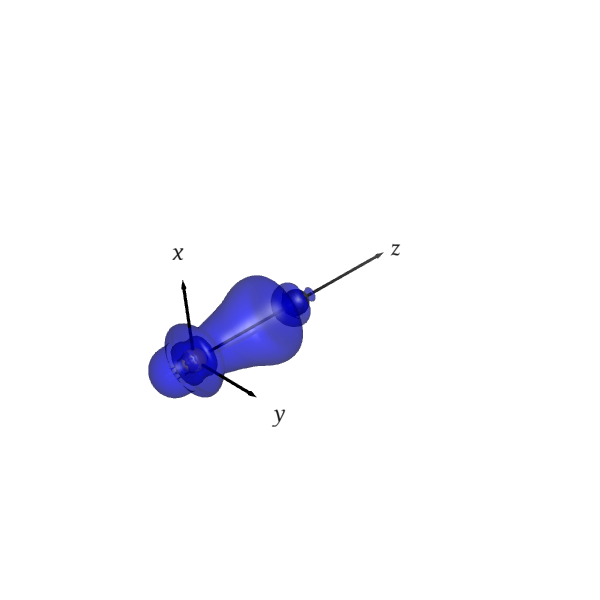
\includegraphics[width=\linewidth]{./AuCn+/nocv+3.png}
        \caption*{\ \ \ \ \ \ \ \ $|\varphi_{+2}|^2$}
    \end{subfigure}
    \hfill
    \begin{subfigure}[t]{0.32\textwidth}
        \centering
        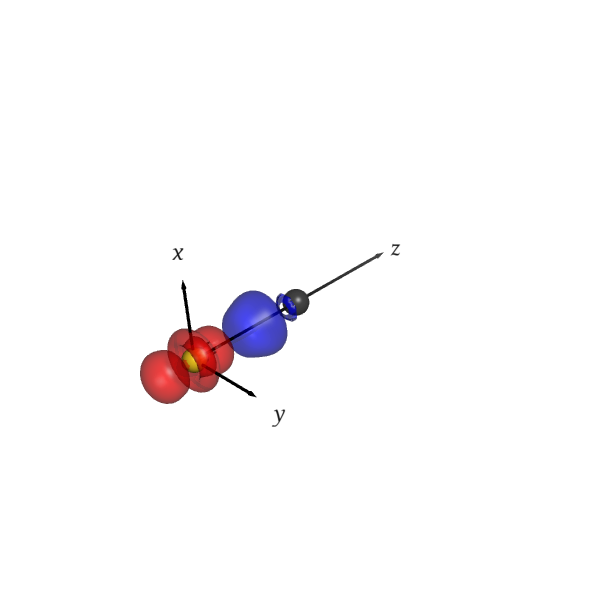
\includegraphics[width=\linewidth]{./AuCn+/pair3.png} 
        \caption*{\ \ \ \ \ \ \ \ $\Delta \rho'_2$} 
    \end{subfigure}

    \vspace{0.0cm}
    \begin{subfigure}[t]{0.32\textwidth}
        \centering
        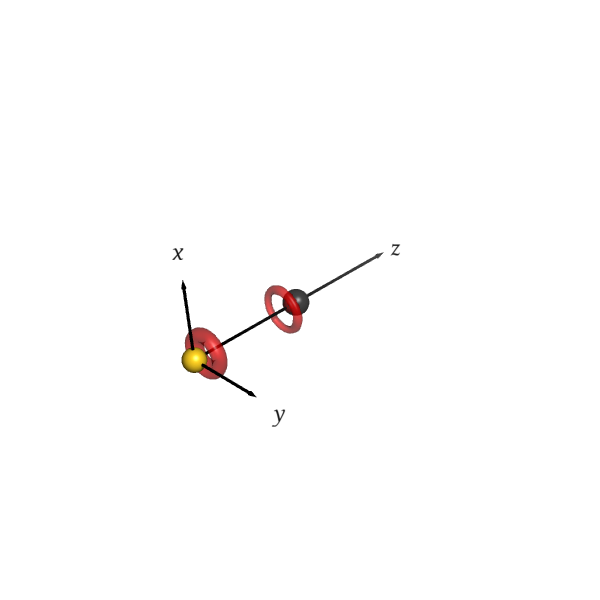
\includegraphics[width=\linewidth]{./AuCn+/nocv-5.png} 
        \caption*{\ \ \ \ \ \ \ \ $|\varphi_{-3}|^2$} 
    \end{subfigure}
    \hfill
    \begin{subfigure}[t]{0.32\textwidth}
        \centering
        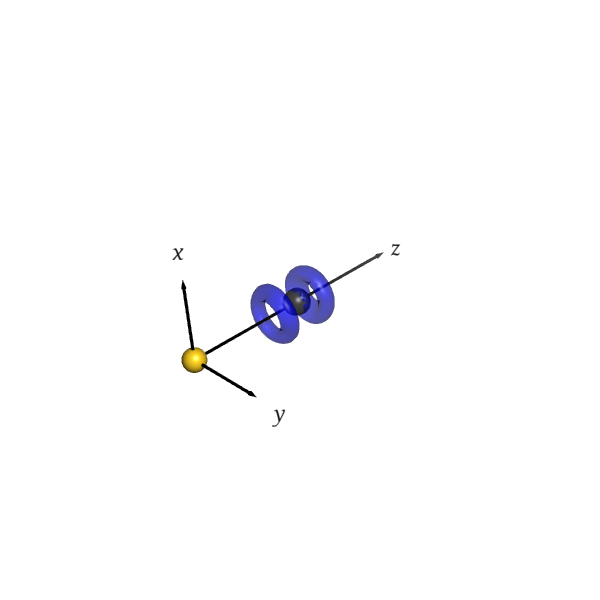
\includegraphics[width=\linewidth]{./AuCn+/nocv+5.png} 
        \caption*{\ \ \ \ \ \ \ \ $|\varphi_{+3}|^2$} 
    \end{subfigure}
    \hfill
    \begin{subfigure}[t]{0.32\textwidth}
        \centering
        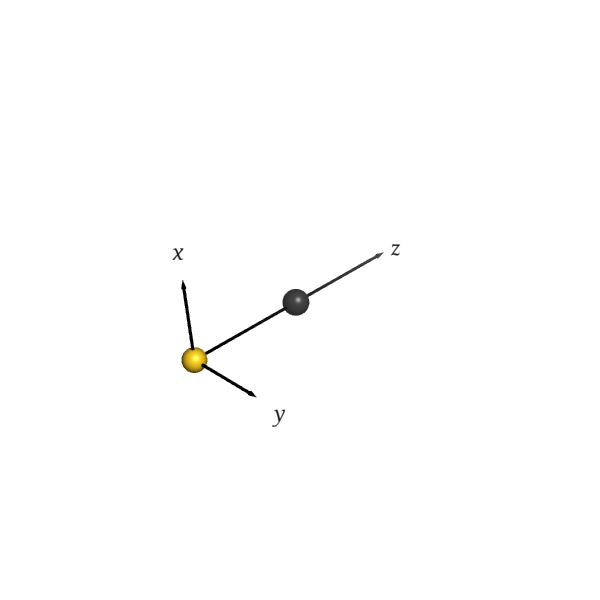
\includegraphics[width=\linewidth]{./AuCn+/pair5.png} 
        \caption*{\ \ \ \ \ \ \ \ $\Delta \rho'_3$} 
    \end{subfigure}

\caption{NOCV pairs for AuCn+ system}
\end{figure}


\begin{figure}[!h]
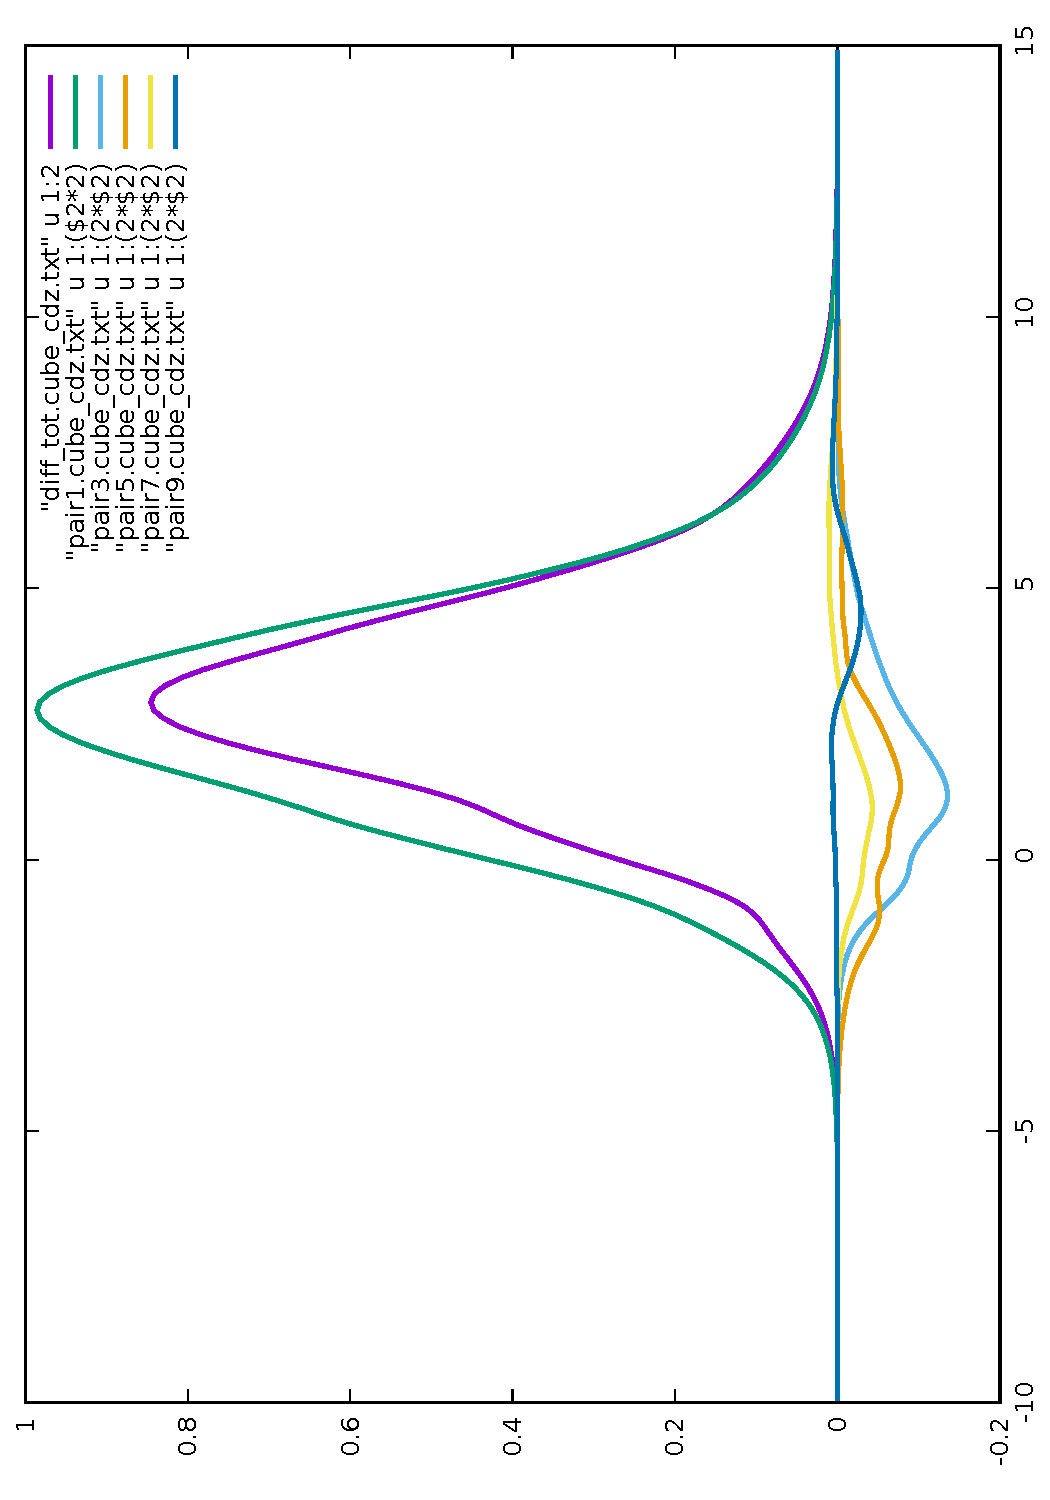
\includegraphics[angle=-90,width=0.80\textwidth]{./AuPb+/cd.pdf}
\caption{CD curve for AuPb+ system}
\end{figure}

\begin{figure}[!h]
    \centering
    \centering
    \begin{subfigure}[t]{0.33\textwidth}
        \centering
        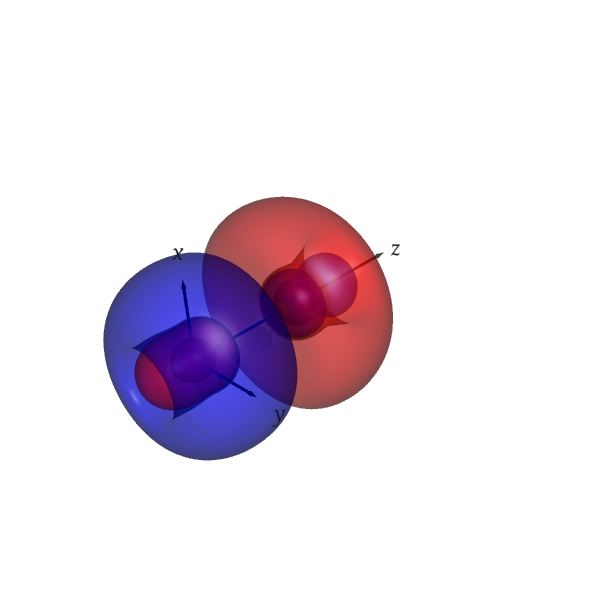
\includegraphics[width=\linewidth]{./AuPb+/diff_tot.png} 
        \caption*{\ \ \ \ \ \ \ \ $\Delta \rho'$} 
    \end{subfigure}
    \hfill
 
    \vspace{0.0cm}
    \begin{subfigure}[t]{0.32\textwidth}
        \centering
        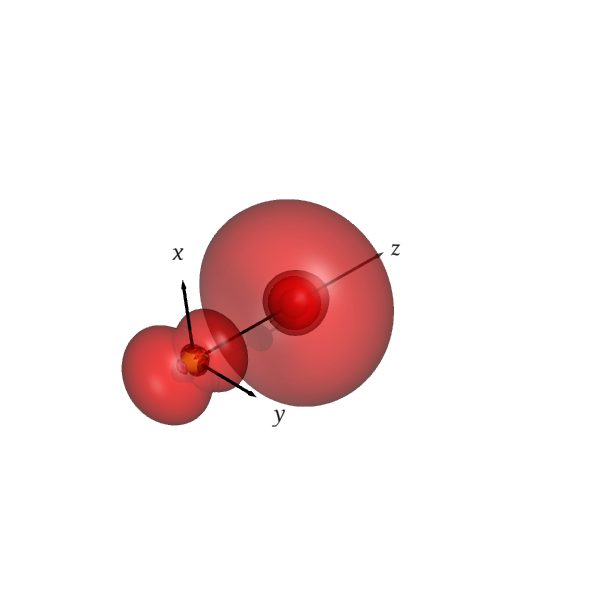
\includegraphics[width=\linewidth]{./AuPb+/nocv-1.png} 
        \caption*{\ \ \ \ \ \ \ \ $|\varphi_{-1}|^2$} 
    \end{subfigure}
    \hfill
    \begin{subfigure}[t]{0.32\textwidth}
        \centering
        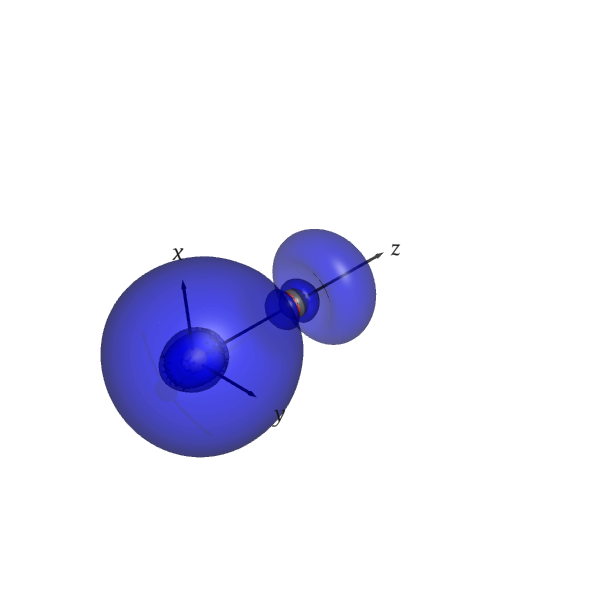
\includegraphics[width=\linewidth]{./AuPb+/nocv+1.png} 
        \caption*{\ \ \ \ \ \ \ \ $|\varphi_{+1}|^2$} 
    \end{subfigure}
    \hfill
    \begin{subfigure}[t]{0.32\textwidth}
        \centering
        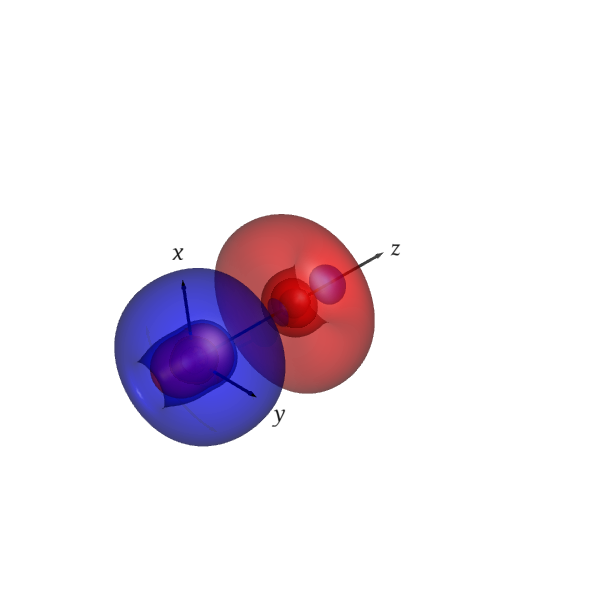
\includegraphics[width=\linewidth]{./AuPb+/pair1.png} 
        \caption*{\ \ \ \ \ \ \ \ $\Delta \rho'_1$} 
    \end{subfigure}

    \vspace{0.0cm}
    \begin{subfigure}[t]{0.32\textwidth}
        \centering
        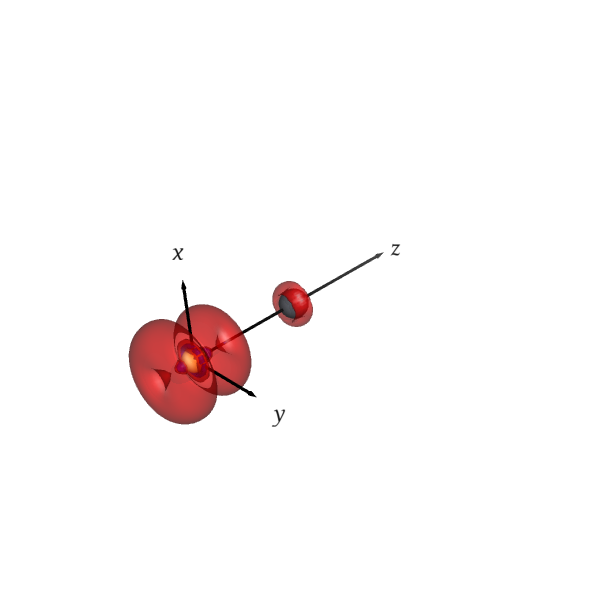
\includegraphics[width=\linewidth]{./AuPb+/nocv-3.png}
        \caption*{\ \ \ \ \ \ \ \ $|\varphi_{-2}|^2$}
    \end{subfigure}
    \hfill
    \begin{subfigure}[t]{0.32\textwidth}
        \centering
        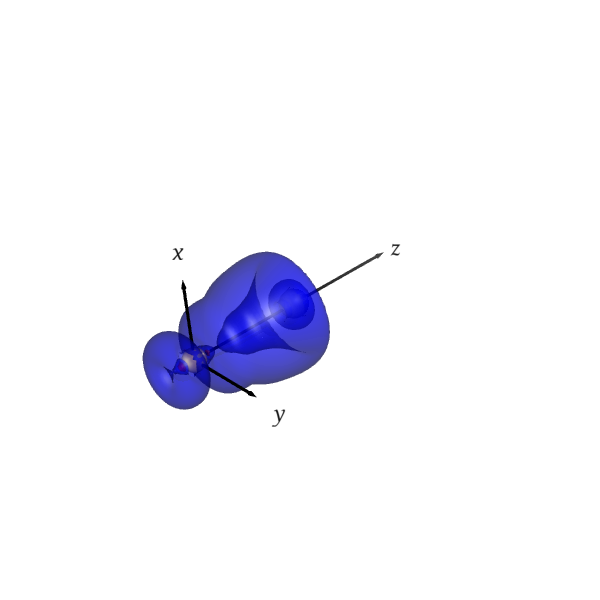
\includegraphics[width=\linewidth]{./AuPb+/nocv+3.png}
        \caption*{\ \ \ \ \ \ \ \ $|\varphi_{+2}|^2$}
    \end{subfigure}
    \hfill
    \begin{subfigure}[t]{0.32\textwidth}
        \centering
        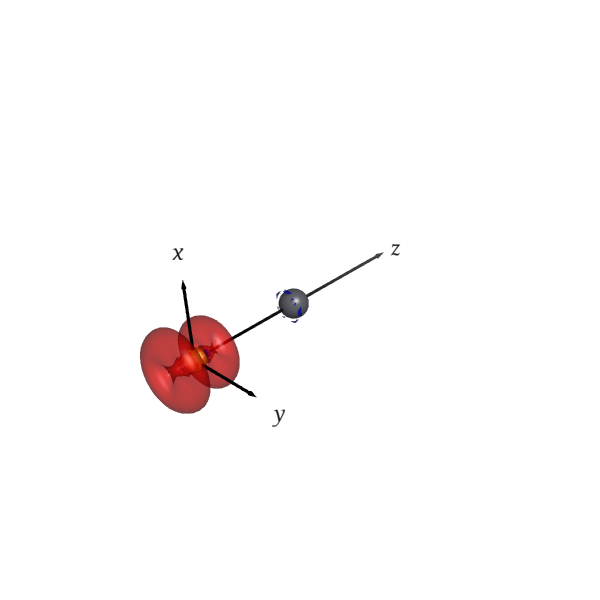
\includegraphics[width=\linewidth]{./AuPb+/pair3.png} 
        \caption*{\ \ \ \ \ \ \ \ $\Delta \rho'_2$} 
    \end{subfigure}

    \vspace{0.0cm}
    \begin{subfigure}[t]{0.32\textwidth}
        \centering
        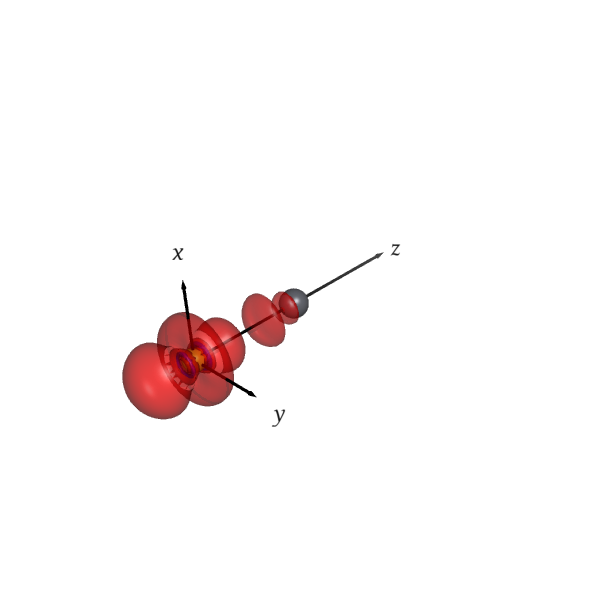
\includegraphics[width=\linewidth]{./AuPb+/nocv-5.png} 
        \caption*{\ \ \ \ \ \ \ \ $|\varphi_{-3}|^2$} 
    \end{subfigure}
    \hfill
    \begin{subfigure}[t]{0.32\textwidth}
        \centering
        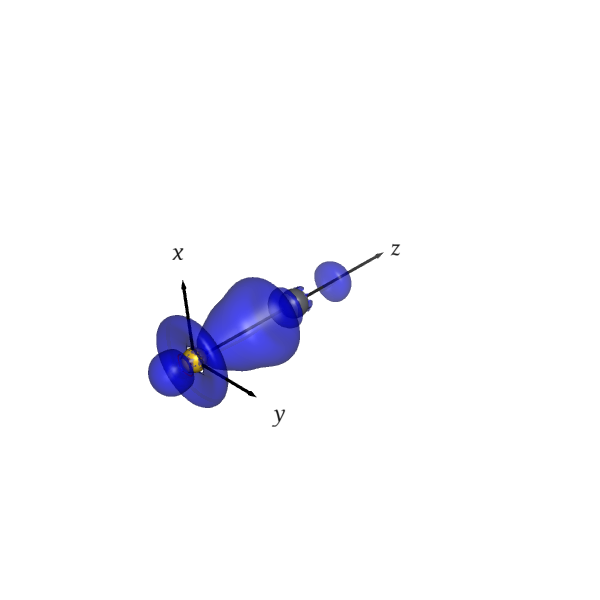
\includegraphics[width=\linewidth]{./AuPb+/nocv+5.png} 
        \caption*{\ \ \ \ \ \ \ \ $|\varphi_{+3}|^2$} 
    \end{subfigure}
    \hfill
    \begin{subfigure}[t]{0.32\textwidth}
        \centering
        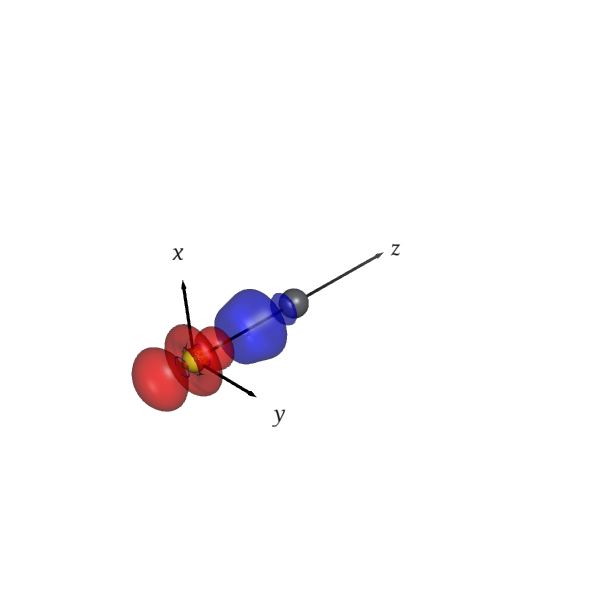
\includegraphics[width=\linewidth]{./AuPb+/pair5.png} 
        \caption*{\ \ \ \ \ \ \ \ $\Delta \rho'_3$} 
    \end{subfigure}

\caption{NOCV pairs for AuPb+ system}
\end{figure}


\begin{figure}[!h]
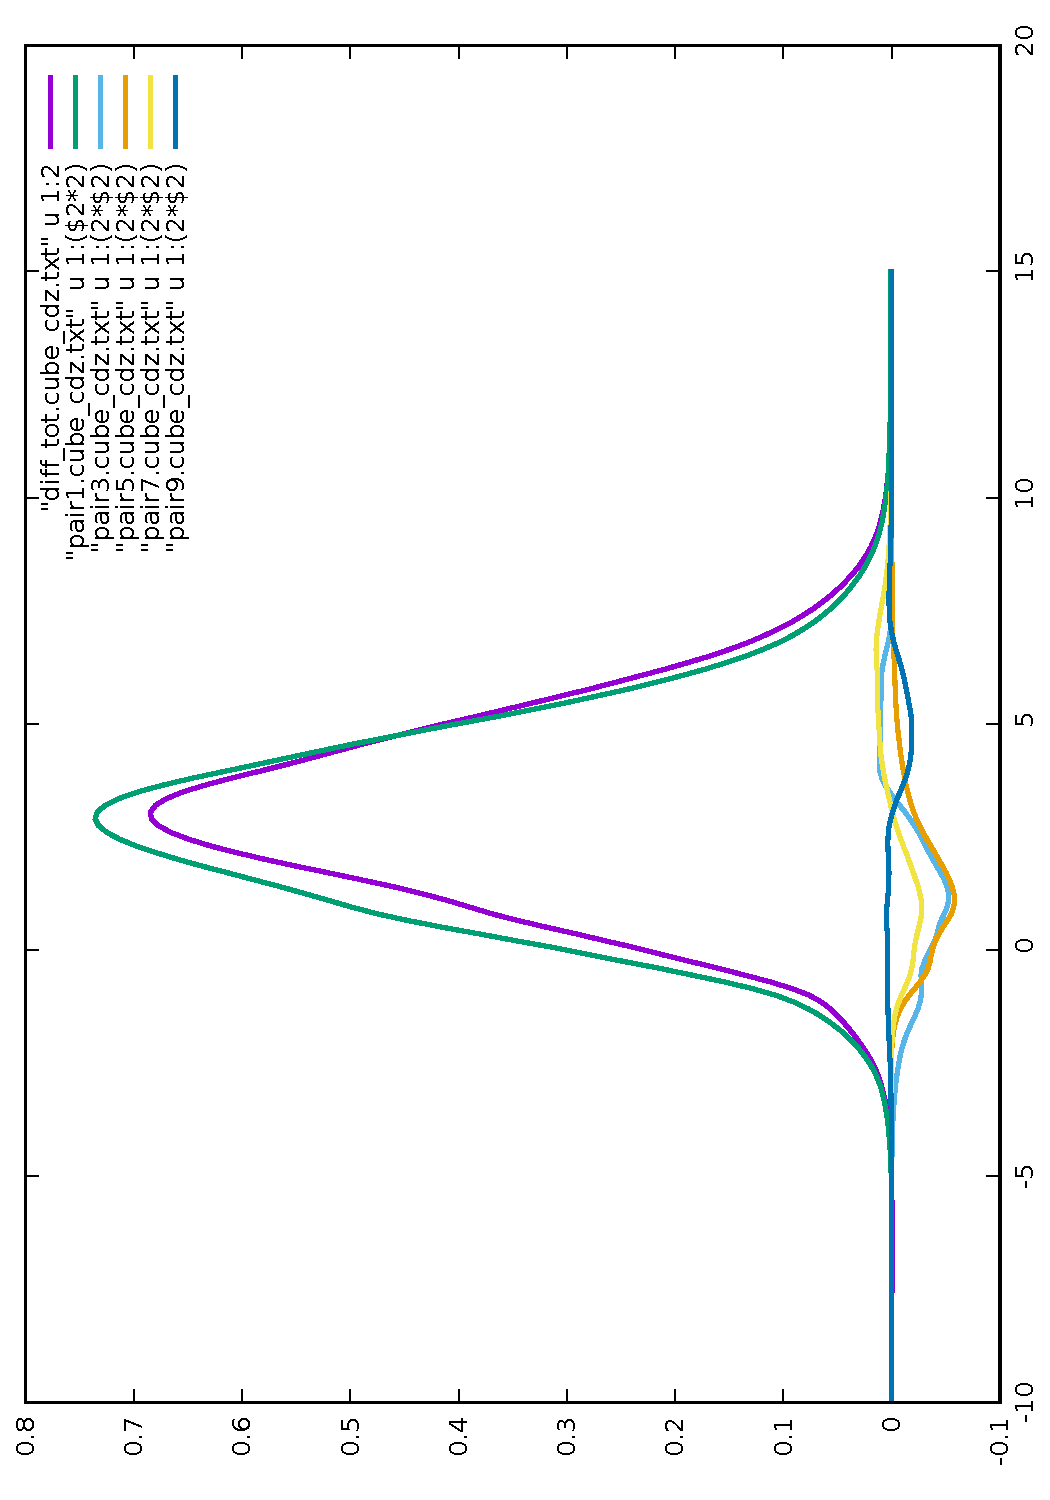
\includegraphics[angle=-90,width=0.80\textwidth]{./AuFl+/cd.pdf}
\caption{CD curve for AuFl+ system}
\end{figure}

\begin{figure}[!h]
    \centering
    \centering
    \begin{subfigure}[t]{0.33\textwidth}
        \centering
        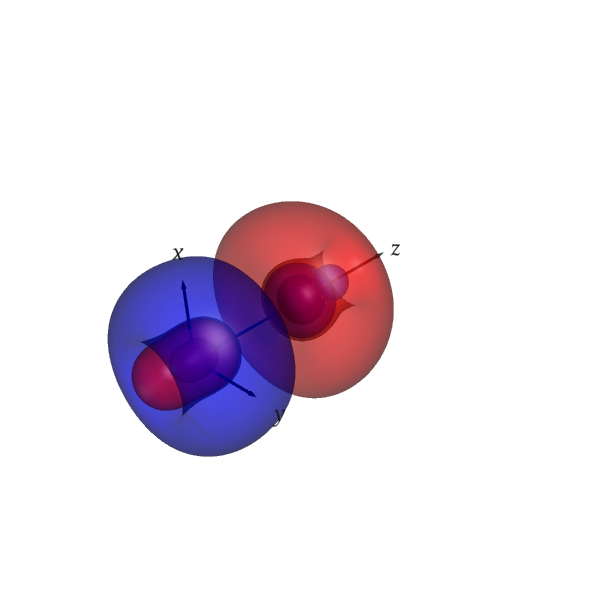
\includegraphics[width=\linewidth]{./AuFl+/diff_tot.png} 
        \caption*{\ \ \ \ \ \ \ \ $\Delta \rho'$} 
    \end{subfigure}
    \hfill
 
    \vspace{0.0cm}
    \begin{subfigure}[t]{0.32\textwidth}
        \centering
        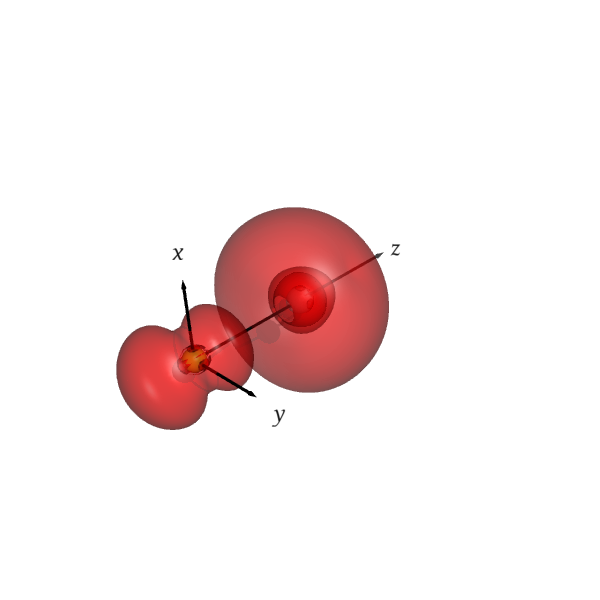
\includegraphics[width=\linewidth]{./AuFl+/nocv-1.png} 
        \caption*{\ \ \ \ \ \ \ \ $|\varphi_{-1}|^2$} 
    \end{subfigure}
    \hfill
    \begin{subfigure}[t]{0.32\textwidth}
        \centering
        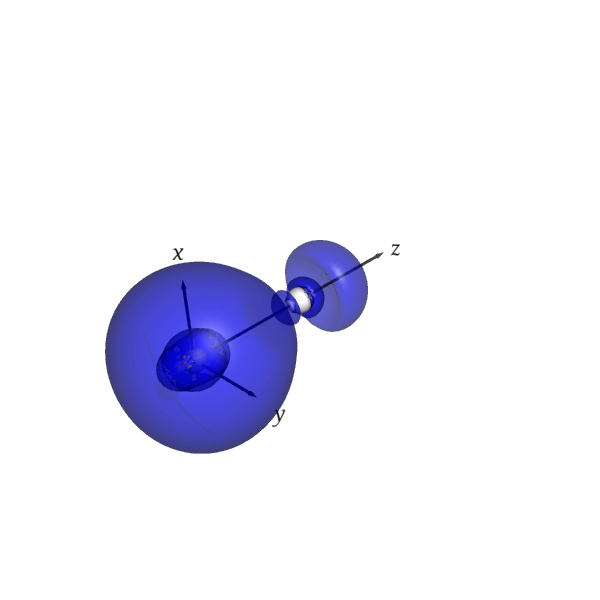
\includegraphics[width=\linewidth]{./AuFl+/nocv+1.png} 
        \caption*{\ \ \ \ \ \ \ \ $|\varphi_{+1}|^2$} 
    \end{subfigure}
    \hfill
    \begin{subfigure}[t]{0.32\textwidth}
        \centering
        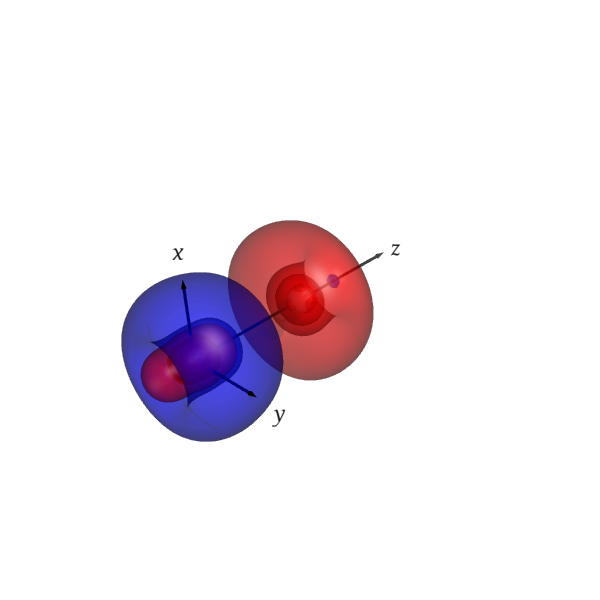
\includegraphics[width=\linewidth]{./AuFl+/pair1.png} 
        \caption*{\ \ \ \ \ \ \ \ $\Delta \rho'_1$} 
    \end{subfigure}

    \vspace{0.0cm}
    \begin{subfigure}[t]{0.32\textwidth}
        \centering
        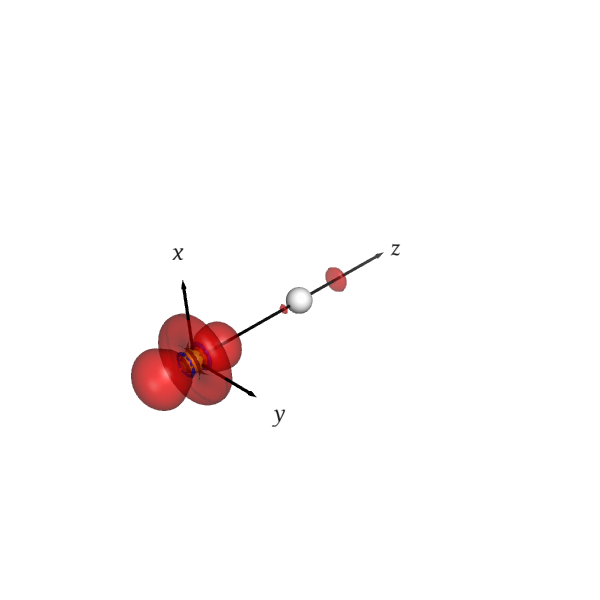
\includegraphics[width=\linewidth]{./AuFl+/nocv-3.png}
        \caption*{\ \ \ \ \ \ \ \ $|\varphi_{-2}|^2$}
    \end{subfigure}
    \hfill
    \begin{subfigure}[t]{0.32\textwidth}
        \centering
        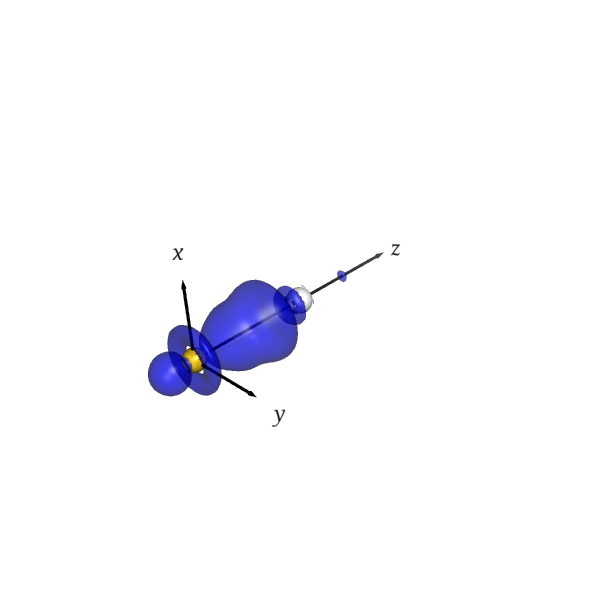
\includegraphics[width=\linewidth]{./AuFl+/nocv+3.png}
        \caption*{\ \ \ \ \ \ \ \ $|\varphi_{+2}|^2$}
    \end{subfigure}
    \hfill
    \begin{subfigure}[t]{0.32\textwidth}
        \centering
        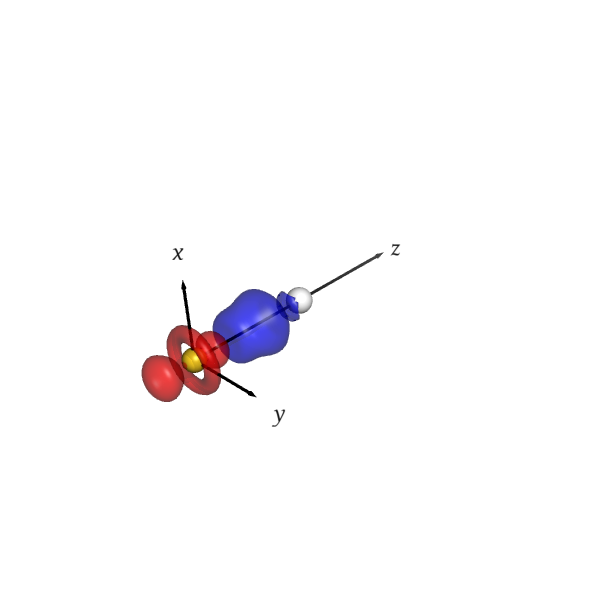
\includegraphics[width=\linewidth]{./AuFl+/pair3.png} 
        \caption*{\ \ \ \ \ \ \ \ $\Delta \rho'_2$} 
    \end{subfigure}

    \vspace{0.0cm}
    \begin{subfigure}[t]{0.32\textwidth}
        \centering
        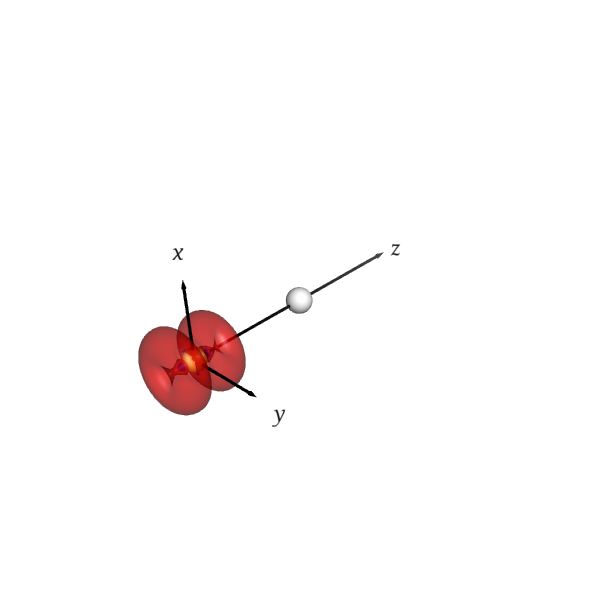
\includegraphics[width=\linewidth]{./AuFl+/nocv-5.png} 
        \caption*{\ \ \ \ \ \ \ \ $|\varphi_{-3}|^2$} 
    \end{subfigure}
    \hfill
    \begin{subfigure}[t]{0.32\textwidth}
        \centering
        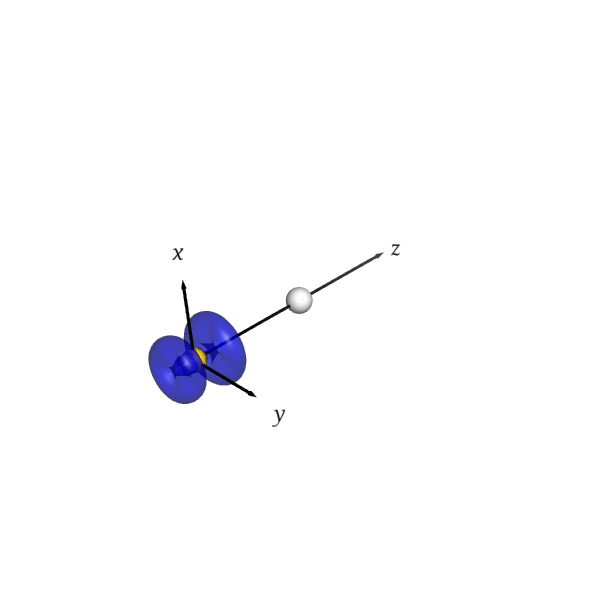
\includegraphics[width=\linewidth]{./AuFl+/nocv+5.png} 
        \caption*{\ \ \ \ \ \ \ \ $|\varphi_{+3}|^2$} 
    \end{subfigure}
    \hfill
    \begin{subfigure}[t]{0.32\textwidth}
        \centering
        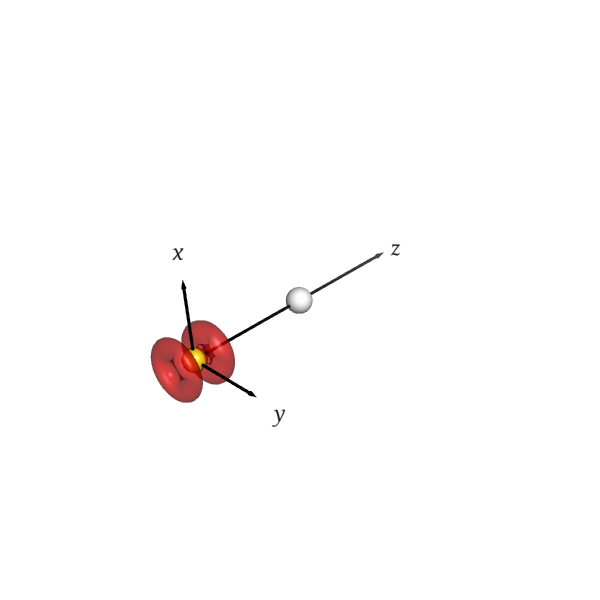
\includegraphics[width=\linewidth]{./AuFl+/pair5.png} 
        \caption*{\ \ \ \ \ \ \ \ $\Delta \rho'_3$} 
    \end{subfigure}

\caption{NOCV pairs for AuFl+ system}
\end{figure}


\begin{figure}[!h]
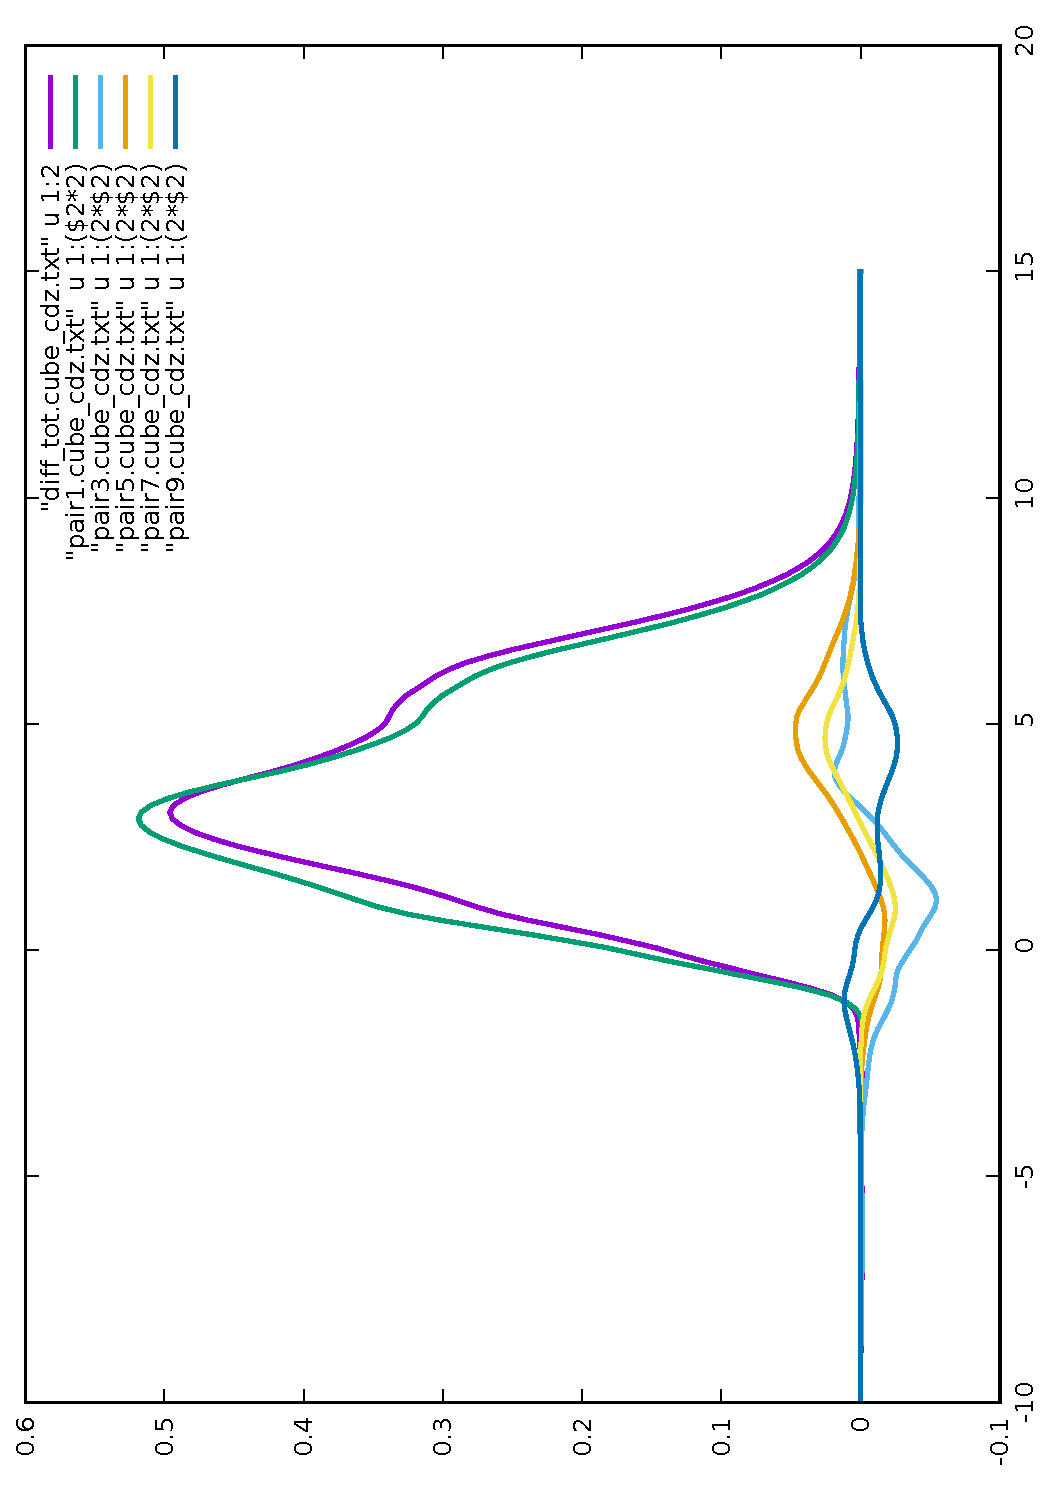
\includegraphics[angle=-90,width=0.80\textwidth]{./AuRn+/cd.pdf}
\caption{CD curve for AuRn+ system}
\end{figure}

\begin{figure}[!h]
    \centering
    \centering
    \begin{subfigure}[t]{0.33\textwidth}
        \centering
        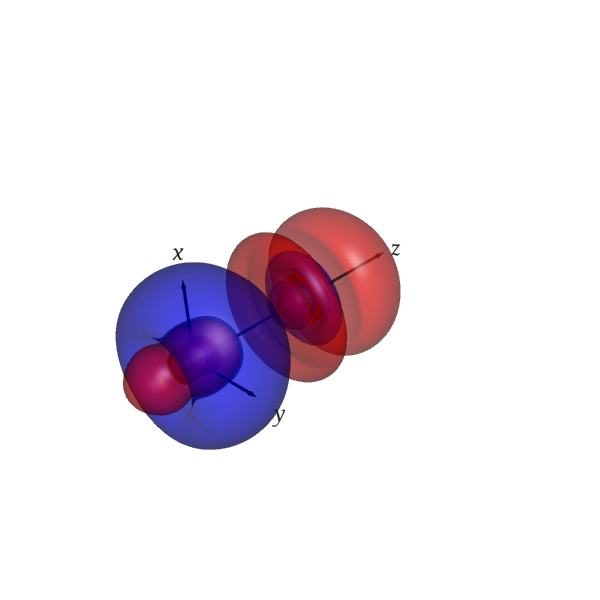
\includegraphics[width=\linewidth]{./AuRn+/diff_tot.png} 
        \caption*{\ \ \ \ \ \ \ \ $\Delta \rho'$} 
    \end{subfigure}
    \hfill
 
    \vspace{0.0cm}
    \begin{subfigure}[t]{0.32\textwidth}
        \centering
        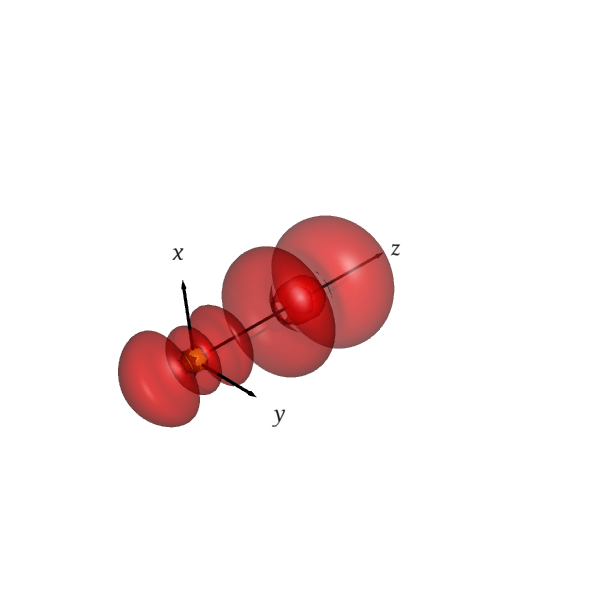
\includegraphics[width=\linewidth]{./AuRn+/nocv-1.png} 
        \caption*{\ \ \ \ \ \ \ \ $|\varphi_{-1}|^2$} 
    \end{subfigure}
    \hfill
    \begin{subfigure}[t]{0.32\textwidth}
        \centering
        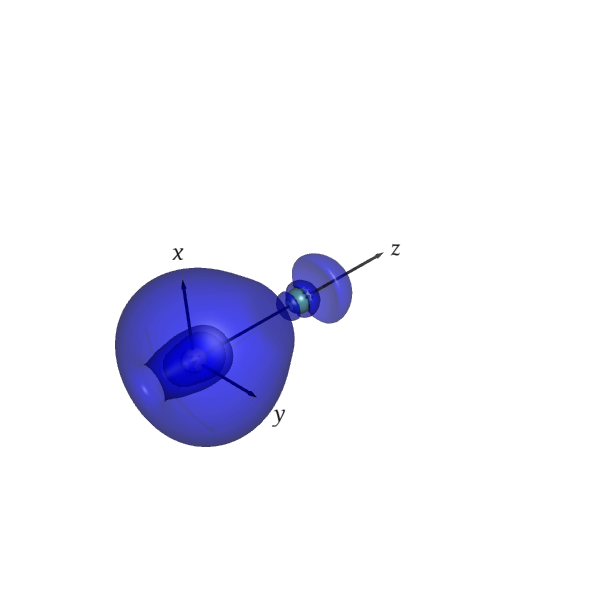
\includegraphics[width=\linewidth]{./AuRn+/nocv+1.png} 
        \caption*{\ \ \ \ \ \ \ \ $|\varphi_{+1}|^2$} 
    \end{subfigure}
    \hfill
    \begin{subfigure}[t]{0.32\textwidth}
        \centering
        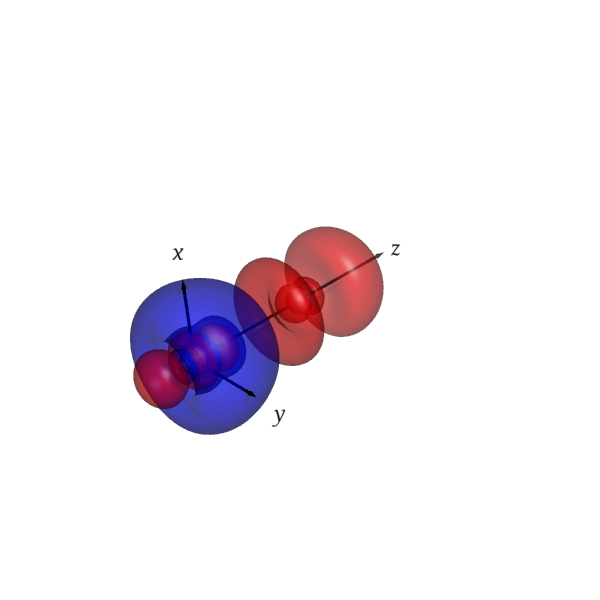
\includegraphics[width=\linewidth]{./AuRn+/pair1.png} 
        \caption*{\ \ \ \ \ \ \ \ $\Delta \rho'_1$} 
    \end{subfigure}

    \vspace{0.0cm}
    \begin{subfigure}[t]{0.32\textwidth}
        \centering
        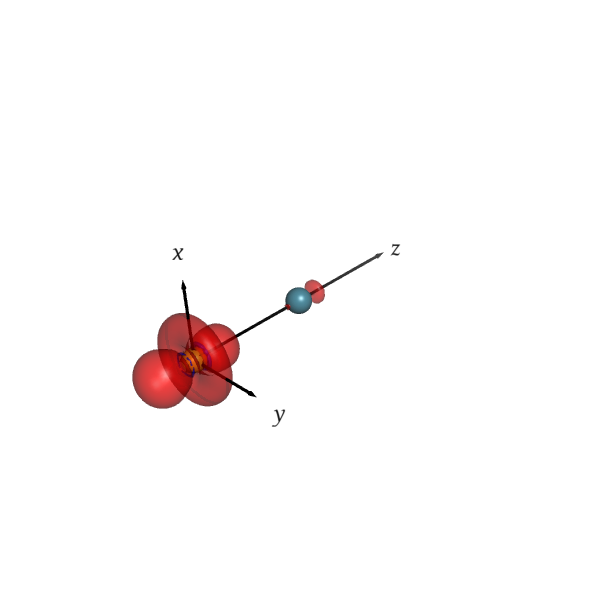
\includegraphics[width=\linewidth]{./AuRn+/nocv-3.png}
        \caption*{\ \ \ \ \ \ \ \ $|\varphi_{-2}|^2$}
    \end{subfigure}
    \hfill
    \begin{subfigure}[t]{0.32\textwidth}
        \centering
        \includegraphics[width=\linewidth]{./AuRn+/nocv+3.png}
        \caption*{\ \ \ \ \ \ \ \ $|\varphi_{+2}|^2$}
    \end{subfigure}
    \hfill
    \begin{subfigure}[t]{0.32\textwidth}
        \centering
        \includegraphics[width=\linewidth]{./AuRn+/pair3.png} 
        \caption*{\ \ \ \ \ \ \ \ $\Delta \rho'_2$} 
    \end{subfigure}

    \vspace{0.0cm}
    \begin{subfigure}[t]{0.32\textwidth}
        \centering
        \includegraphics[width=\linewidth]{./AuRn+/nocv-5.png} 
        \caption*{\ \ \ \ \ \ \ \ $|\varphi_{-3}|^2$} 
    \end{subfigure}
    \hfill
    \begin{subfigure}[t]{0.32\textwidth}
        \centering
        \includegraphics[width=\linewidth]{./AuRn+/nocv+5.png} 
        \caption*{\ \ \ \ \ \ \ \ $|\varphi_{+3}|^2$} 
    \end{subfigure}
    \hfill
    \begin{subfigure}[t]{0.32\textwidth}
        \centering
        \includegraphics[width=\linewidth]{./AuRn+/pair5.png} 
        \caption*{\ \ \ \ \ \ \ \ $\Delta \rho'_3$} 
    \end{subfigure}

\caption{NOCV pairs for AuRn+ system}
\end{figure}


\begin{figure}[!h]
\includegraphics[angle=-90,width=0.80\textwidth]{./AuOg+/cd.pdf}
\caption{CD curve for AuOg+ system}
\end{figure}

\begin{figure}[!h]
    \centering
    \centering
    \begin{subfigure}[t]{0.33\textwidth}
        \centering
        \includegraphics[width=\linewidth]{./AuOg+/diff_tot.png} 
        \caption*{\ \ \ \ \ \ \ \ $\Delta \rho'$} 
    \end{subfigure}
    \hfill
 
    \vspace{0.0cm}
    \begin{subfigure}[t]{0.32\textwidth}
        \centering
        \includegraphics[width=\linewidth]{./AuOg+/nocv-1.png} 
        \caption*{\ \ \ \ \ \ \ \ $|\varphi_{-1}|^2$} 
    \end{subfigure}
    \hfill
    \begin{subfigure}[t]{0.32\textwidth}
        \centering
        \includegraphics[width=\linewidth]{./AuOg+/nocv+1.png} 
        \caption*{\ \ \ \ \ \ \ \ $|\varphi_{+1}|^2$} 
    \end{subfigure}
    \hfill
    \begin{subfigure}[t]{0.32\textwidth}
        \centering
        \includegraphics[width=\linewidth]{./AuOg+/pair1.png} 
        \caption*{\ \ \ \ \ \ \ \ $\Delta \rho'_1$} 
    \end{subfigure}

    \vspace{0.0cm}
    \begin{subfigure}[t]{0.32\textwidth}
        \centering
        \includegraphics[width=\linewidth]{./AuOg+/nocv-3.png}
        \caption*{\ \ \ \ \ \ \ \ $|\varphi_{-2}|^2$}
    \end{subfigure}
    \hfill
    \begin{subfigure}[t]{0.32\textwidth}
        \centering
        \includegraphics[width=\linewidth]{./AuOg+/nocv+3.png}
        \caption*{\ \ \ \ \ \ \ \ $|\varphi_{+2}|^2$}
    \end{subfigure}
    \hfill
    \begin{subfigure}[t]{0.32\textwidth}
        \centering
        \includegraphics[width=\linewidth]{./AuOg+/pair3.png} 
        \caption*{\ \ \ \ \ \ \ \ $\Delta \rho'_2$} 
    \end{subfigure}

    \vspace{0.0cm}
    \begin{subfigure}[t]{0.32\textwidth}
        \centering
        \includegraphics[width=\linewidth]{./AuOg+/nocv-5.png} 
        \caption*{\ \ \ \ \ \ \ \ $|\varphi_{-3}|^2$} 
    \end{subfigure}
    \hfill
    \begin{subfigure}[t]{0.32\textwidth}
        \centering
        \includegraphics[width=\linewidth]{./AuOg+/nocv+5.png} 
        \caption*{\ \ \ \ \ \ \ \ $|\varphi_{+3}|^2$} 
    \end{subfigure}
    \hfill
    \begin{subfigure}[t]{0.32\textwidth}
        \centering
        \includegraphics[width=\linewidth]{./AuOg+/pair5.png} 
        \caption*{\ \ \ \ \ \ \ \ $\Delta \rho'_3$} 
    \end{subfigure}

\caption{NOCV pairs for AuOg+ system}
\end{figure}


\section{A case study the ClAuX (X=Hg, Pb, Rn, Cn, Fl, Og) systems  }


Insert basis set and fitting set used 


\section{Conclusions}

\end{document}
